\iffalse
\documentclass[journal,10pt,twocolumn]{article}
\usepackage{graphicx, float}
\usepackage[margin=0.5in]{geometry}
\usepackage{amsmath, bm}
\usepackage{array}
\usepackage{booktabs}
\usepackage{xfrac}

\providecommand{\norm}[1]{\left\lVert#1\right\rVert}
\let\vec\mathbf
\newcommand{\myvec}[1]{\ensuremath{\begin{pmatrix}#1\end{pmatrix}}}
\newcommand{\mydet}[1]{\ensuremath{\begin{vmatrix}#1\end{vmatrix}}}

\title{\textbf{Line Assignment}}
\author{Harsha sai sampath kumar}
\date{September 2022}

\begin{document}

\maketitle
\paragraph{\textit{\large Problem Statement} -
\fi
Find the equation of the line through the point (0,2) making an angle \begin{align}2\pi/3\end{align} with the positive X-axis. Also find the equation of the line parallel to it and crossing the Y-axis at a distance of 2 units below the origin
	\begin{figure}[!ht]
		\centering
 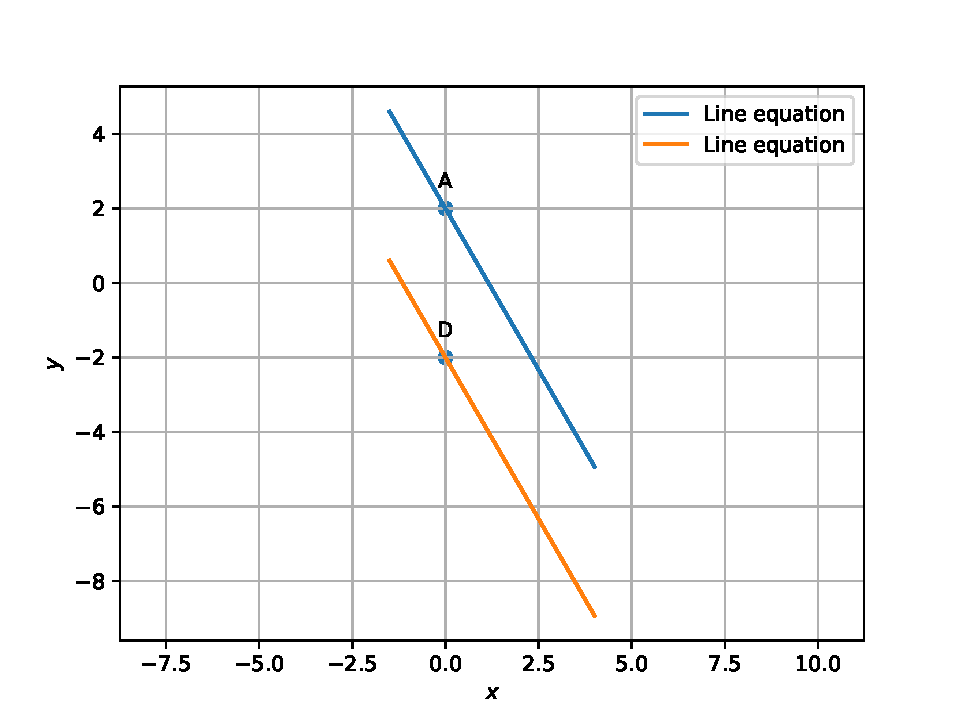
\includegraphics[width=\columnwidth]{chapters/11/10/2/14/figs/fig.pdf}
		\caption{}
		\label{fig:11/10/2/14}
  	\end{figure}
	\\
	\solution
\iffalse
	}

\section*{\large Solution}

\begin{figure}[H]
\centering
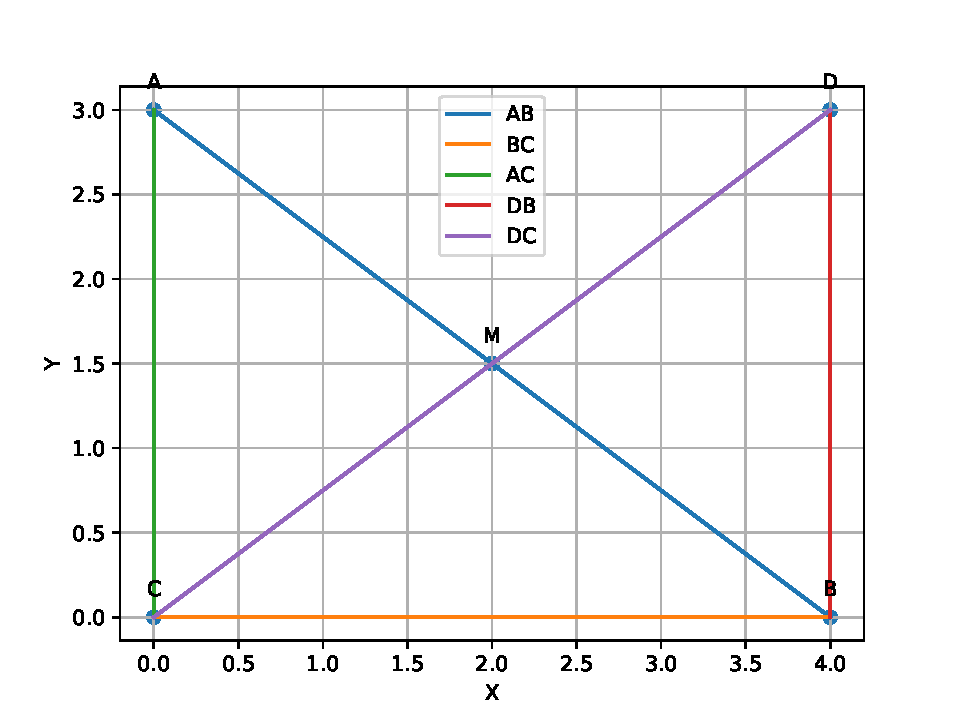
\includegraphics[width=1\columnwidth]{fig.pdf}
\caption{}
\end{figure}


\section{construction}

\begin{tabular}{|c|c|}
	\hline
	\textbf{Point}&\textbf{Value}\\
	\hline
	A&\myvec{0\\2}\\
	\hline
	$\theta$&2$\pi$/3\\
	\hline
	D&\myvec{0\\-2}\\
	\hline
	
	
\end{tabular}


\section*{Assumptions}
To find the line equation  through the point (0,2)
\vspace*{3mm}
\fi
From the  given information, the direction vector is
\begin{align}
	\vec{m}=\myvec{1\\-\sqrt{3}}
\end{align}
  
Thus, 
the normal vector is
\begin{align}
	\vec{n}=\myvec{\sqrt{3}\\1}
\end{align}

\iffalse
\begin{align}
	\vec{m}=\myvec{1\\-\sqrt{3}}
	\vec{n}=\myvec{\sqrt{3}\\1}
\end{align}


\begin{align}
	\vec{n^T}=(\sqrt{3}&1)	
\end{align}






Where line equation  is given by:
\begin{align}
\vec{n^T(x-p)}=0
\label{pf2-eq-1}
\end{align}

By substituting the values in the above equation:
\fi
and the 
equation of the line is 
\begin{align}
	\myvec{\sqrt{3} &1}\myvec{\vec{x}-\myvec{0\\2}}&=0
	\\
	\implies 
	\myvec{\sqrt{3}&1}
	\vec{x}&=2
\end{align}
The equation of the parallel crossing the Y-axis at a distance of 2 units below the origin is given by 
\begin{align}
	\myvec{\sqrt{3} &1}\myvec{\vec{x}-\myvec{0\\-2}}&=0
	\\
	\implies 
	\myvec{\sqrt{3}&1}
\vec{x}=-2
\end{align}
